\chapter{Trajectory planning and control of quadrotors under wind}

Navigation of a quadrotor in outdoor environments where wind disturbances affect the quadrotor is an active area of research. Solving the problem of safe quadrotor navigation in the presence of wind disturbances involves various aspects of existing methods for quadrotor navigation and wind disturbance rejection, and in particular presents the challenge of extending existing methods. In this chapter, an overview of the state of the art is presented to show where one can enter and extend the existing literature. This chapter points out drawbacks of existing methods and presents the problem formulation that was found to solve the existing disadvantages.

\section{Background}

To get to the problem statement and describe the ways in which this thesis will expand upon the existing literature, a brief overview of the current state of the art is provided. A review of current motion planners and controllers commonly used for quadrotor control is presented. It is discussed how these are extended to deal with wind disturbances and uncertainties in the classical approach and using new data-driven and machine learning methods. 
 
\subsection{Standard flight trajectory planning and control}

A quadrotor is the most typical MAV that consists of a rigid body with four rotors. By varying the power of the rotors, the quadrotor can perform various flight maneuvers, such as hovering, ascending, descending, and rotating about its axes. Navigating a quadrotor often involves not only controlling its motion, but also planning a feasible sequence of movements to get from one point to another. The motion planner precedes the quadrotor controller, and ideally both parts take into account the dynamics of the quadrotor and possible external disturbances. 

The goal of the motion planner is to find a valid motion sequence of the quadrotor from its start position to the goal position, without colliding with obstacles in the environment. Motion planners can be divided into \textit{global} planners and \textit{local} planners. Global planners plan the entire motion sequence from start to end position using a map of the environment. Local planners update waypoints as the quadrotor moves, taking into account dynamic obstacles and vehicle constraints. Another distinction is made between \textit{path} planners and \textit{trajectory} planners. Path planners ignore the dynamics of the quadrotor and other differential constraints. They focus primarily on the translations and rotations required to move the robot. Common path planners are search-based methods, sampling-based methods and potential field methods \cite{quan2020survey}. 

However, if the robot is subject to dynamics:
\begin{equation}
\dot{\mathbf{x}}=f(\mathbf{x}, \mathbf{u})
\end{equation}
with mechanical constraints on the state space $\mathbf{x} \in \mathcal{X}$ and input space $\mathbf{u} \in \mathcal{U}$, these must be considered in the motion planning problem. This is called the trajectory planning problem, where the trajectory describes the evolution of vehicle configurations over time. Usually, the path planner precedes the trajectory planner, which then time-parameterizes the solutions of the path planner \cite{goerzen2010survey}. Some trajectory planners also solve both problems simultaneously. The existing approaches for quadrotor trajectory planning can mainly be divided into polynomial approaches, discrete-time search methods, sampling-based approaches and optimization methods \cite{penicka2022minimum}.

The quadrotor motion is typically controlled in a cascaded control structure as shown in Figure \ref{fig::controlarchitecture}. It consists of an outer loop position controller and an inner loop attitude controller. The position controller computes the desired attitude angles of the quadrotor to reach a certain position $\mathbf{p}_d$ and rotation $\psi_d$. The attitude controller tracks the desired roll, pitch and yaw $\phi_d$,$\theta_d$,$\psi_d$ by controlling the angular velocity $\dot{\phi}_d$,$\dot{\theta}_d$,$\dot{\psi}_d$ and thrust $T_d$ needed to keep the quadrotor in the air. The mixer is in place to translate the angular velocities and thrust command into individual rotor commands. 

\begin{figure}[htb!]
    \centering
    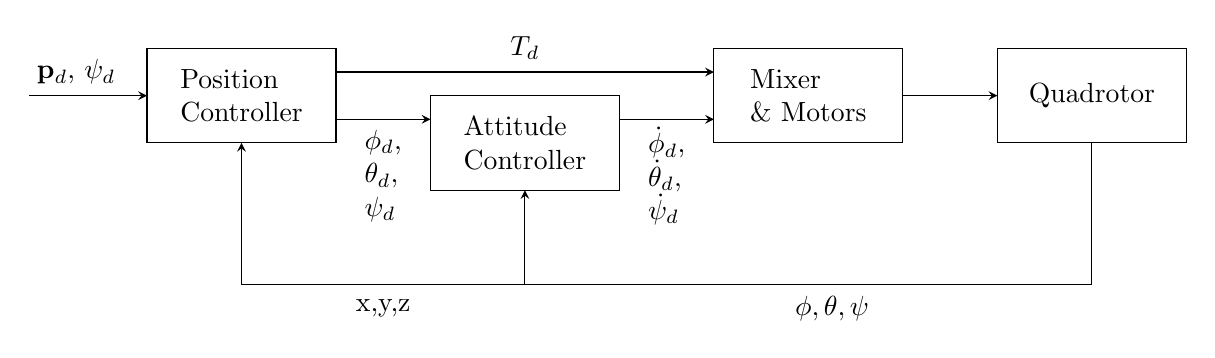
\begin{tikzpicture}[scale = 0.6]
        \draw  (-2,-0.5) rectangle (2,-2.5);
        \node[align=left] at (0,-1.5) {Attitude\\Controller};
        
        \draw  (4,0.5) rectangle (8,-1.5);
        \draw  (-4,0.5) rectangle (-8,-1.5);
        \draw [-stealth] (-4,0) -- (4,0);
        \draw  [-stealth] (-4,-1) -- (-2,-1);
        \draw  [-stealth](2,-1) -- (4,-1);
        \draw  (10,0.5) rectangle (14,-1.5);
        \draw  [-stealth](8,-0.5) -- (10,-0.5);
        \draw  [-stealth](12,-1.5) -- (12,-4.5) -- (0,-4.5) node (v1) {} -- (0,-2.5);
        \draw  [-stealth](0,-4.5) -- (-6,-4.5) -- (-6,-1.5);
        \draw  [-stealth](-10.5,-0.5) -- (-8,-0.5);
        \node[align=left] at (-6,-0.5) {Position\\Controller};
        \node[align=left] at (6,-0.5) {Mixer\\ \& Motors};
        \node at (12,-0.5) {Quadrotor};
        \node at (6.5,-5) {$\phi, \theta, \psi$};
        \node at (-3,-5) {x,y,z};
        \node[align=left] at (-3,-2.2) {$\phi_d$,\\$\theta_d,$\\  $\psi_d$};
        \node[align=left] at (3,-2.2) {$\dot{\phi}_d$,\\$\dot{\theta}_d,$\\  $\dot{\psi}_d$};
        \node at (0,0.5) {$T_d$};
        \node at (9,0) {};
        \node at (-9.5,0) {$\mathbf{p}_d$, $\psi_d$};
    \end{tikzpicture}
    \caption{Cascaded control architecture of a common quadrotor controller.}
    \label{fig::controlarchitecture}
\end{figure}

Due to the increased research interest in quadrotors in the last decades, numerous control techniques have been implemented for the quadrotor, ranging from linear to nonlinear control methods, model-based versus model-free controllers, robust, adaptive, and intelligent controllers (e.g.. \cite{nascimento2019position}, \cite{zulu2016review}, \cite{emran2018review}, \cite{li2015survey}, \cite{kendoul2012survey}).
Linear controllers are applicable where the quadrotor does not deviate significantly from the hovering state. For extreme flight manoeuvres, e.g. racing, or when controlling the attitude of the quadrotor, non-linear control methods are typically used \cite{nguyen2021model}.  

When a model of the quadrotor dynamics is available, model-based methods provide a way to incorporate the system dynamics into the controller design and facilitate tuning of the control parameters. Among model-based methods, Model Predictive Control (MPC) is a popular method for quadrotor control. MPC \cite{rawlings2017model} solves an optimal control problem (OCP) on-line at each sampling instant taking the current state of the plant as the initial state. Based on the system model, it predicts the future evolution of the states over a finite horizon. With the known system evolution, it optimizes for a sequence of control inputs, given a certain cost. After obtaining the optimal control sequence, only the first control input is applied to the system. At the subsequent time-step, the OCP is solved with the new current state. The formulation of the OCP allows to directly impose constraints on the system, which is one of the major advantages of MPC over other control methods. 

With optimization-based methods, it is also possible to combine both trajectory planning and trajectory tracking in one optimization problem. Given a path by the planner, the optimization problem solves for the optimal system states and system inputs. The key to solving this problem is to use an MPC algorithm that is modified to simultaneously solve the trajectory generation problem. One popular method to achieve this is Model Predictive Contouring Control (MPCC) \cite{lam2010model}. MPCC has been applied for static and dynamic obstacle avoidance with ground vehicles \cite{schwarting2017safe} and autonomous ground robots \cite{brito2019model}. In the context of quadrotor navigation it has found an application in quadrotor racing \cite{romero2021model}.

%Navigating a quadrotor in the conventional case can be categorized into four steps: 

%\begin{figure}[htb!]
%     \centering
%     \begin{tikzpicture}
    
%     \draw  (-3.5,1) rectangle (-0.5,-1);
%     \draw  (0.5,1) rectangle (3.5,-1);
%     \draw  (4.5,1) rectangle (7.5,-1);
%     \draw  (8.5,1) rectangle (11.5,-1);
%     \node[align=left] at (-2,0) {Motion\\Planner};
%     \node[align=left] at (2,0) {Position\\Control};
%     \node[align=left] at (6,0) {Attitude\\Control};
%     \node[align=left] at (10,0) {Mixer};
%     \draw [-stealth] (-0.5,0) -- (0.5,0);
%     \draw [-stealth] (3.5,0) -- (4.5,0);
%     \draw [-stealth] (7.5,0) -- (8.5,0);
%     \end{tikzpicture}
%     \caption{Commonly used control structure of the motion planner and controller.}
%     \label{fig::soaMP}
% \end{figure}

% \begin{enumerate}
%     \item The motion planner, that sends the desired trajectory to the position controller.
%     \item The position controller that gives Euler angles as a reference to the attitude controller.
%     \item The attitude controller that controls the orientation of the robot on its three Euler angular velocities and the desired thrust.
%     \item The mixer, that translates the angular velocities and thrust command into individual rotor commands. 
% \end{enumerate}

\subsection{Dealing with wind disturbances}

In many practical applications, the quadrotor is subject to external wind disturbances. The wind field may vary in time and space, which must be considered in the motion planning and control design. 

There are several control algorithms that observe the disturbance online and reject it by calculating a compensating control input. If the drone is equipped with airspeed sensors such as Pitot tubes, a local estimate of the wind can be determined directly \cite{sydney2013dynamic}. In most cases, however, these sensors are not present on board the quadrotor. Instead, one could use the model of the quadrotor to estimate the wind based on the difference between desired and measured velocity or acceleration. This idea was used, e.g. for a nonlinear inversion-based position controller in \cite{smeur2018cascaded}. The authors in \cite{tomic2014unified} use an observer design to estimate the external force vectors. However, this method only provides a deterministic estimate of the disturbance. More information about the disturbance can be obtained using stochastic estimators such as the extended or unscented Kalman filter \cite{hentzen2019disturbance}. In addition to the nominal disturbance force or nominal disturbance torque, these estimators also provide an uncertainty of the estimate that can be incorporated into the controller design. 

In motion planning and predictive control it is advantageous to know the evolution of the disturbance over future states. One way to accomplish this is to have a comprehensive aerodynamic model to describe wind disturbances \cite{waslander2009wind}. A drawback is that determining the model parameters requires extensive experimentation, and incorporating the complex model into a predictive controller increases the computational cost. In addition, robust methods have been developed \cite{ton2012robust} that assume a constant disturbance bound for all future states, and guarantee performance for all disturbances within this bound. 

In particular, robust motion planning algorithms have been active areas of research in the past few years. \cite{kousik2020bridging}. A way to introduce robustness into the motion planner are reachability-based methods, taking into account all possible states that the quadrotor can reach, given information about its uncertainty. The authors in \cite{majumdar2017funnel} precompute a library of safety funnels around trajectories, which are pieced together at runtime to generate feasible and safe trajectories. Furthermore, Hamilton-Jacobi (HJ) reachability analysis was developed for robust offline trajectory planning in fully known environments and independent of the motion planner, called FasTrack \cite{herbert2017fastrack}. FasTrack computes the tracking error as a function of control inputs and generates a feedback controller to compensate for it. The work presented by the authors in \cite{kousik2020bridging} uses forward reachable sets (FRS) that bound the tracking error and are computed offline. During online planning, the FRS are used to map obstacles to parameterized trajectories so that a safe trajectory can be selected. The authors in \cite{wu2021external} use FRS to compute outer bounding ellipsoids that approximate the position of the quadrotor plus its uncertainty, which are then used in an NMPC controller (see Figure \ref{fig::external}).

NMPC methods are leveraged for robust motion planning and control algorithms that can deal with both set-bounded and probabilistic uncertainties. Robust MPC formulations are used, e.g., by the robust collision avoidance problem in \cite{kamel2017linear}. Additionally, the authors in \cite{singh2019robust} build on the idea of robust MPC and use control contraction metrics to design a feedback control law and tube. Stochastic MPC formulations for collision and obstacle avoidance were initially presented by the authors in \cite{blackmore2011chance}, where polytopic chance constraints were reformulated into deterministic constraints. This work was extended with quadratic obstacle avoidance constraints for dynamic collision avoidance \cite{zhu2019chance}. 
% The authors in \cite{hewing2019cautious} combine robust and stochastic methods by using a feedback controller and probabilistic reachable sets to reformulate chance constraints. However, this work is limited to linear systems. 

\subsection{Data-driven disturbance model}

Data-driven disturbance estimation and rejection and more detailed disturbance models can be combined into data-driven disturbance models. Data-driven modelling techniques have been developed to improve existing system models for a variety of applications. 

A prominent method for learning a robust representation of the model uncertainty is set-membership identification \cite{lorenzen2019robust}, \cite{didier2021adaptive}. A practical implementation of set-membership identification together with model predictive control on a quadrotor is presented by the authors in \cite{didier2021robust}. Using set-membership identification, the drone is able to adapt parameters in uncertain wind conditions, while satisfying the constraints \cite{didier2021robust}. 

The authors in \cite{o2021meta} use meta-learning with a deep neural network to model the residual dynamics associated with wind disturbances on a quadrotor platform.

Furthermore, Gaussian processes (TODO: cite) models are used learn a stochastic model of the dynamics. In the context of quadrotor control, GPs have been used to describe the nonlinear dynamics and aerodynamic effects during aggressive flight maneuvers \cite{torrente2021data} and to guarantee robust obstacle avoidance \cite{garimella2017robust}. Furthermore GPs are used to model wind uncertainties in \cite{mehndiratta2020gaussian}. Three independent GPs are trained based on the observed disturbances. Therefore, the approach can only respond to disturbances if they have been observed. The work in \cite{tagliabue2021airflow} creates a wind map based on the quadrotor position fusing Inertial Measurement Unit (IMU) and airflow measurements. Moreover, Gaussian processes have been used successfully to model residual dynamics for mobile robots \cite{ostafew2016robust}, race cars \cite{kabzan2019learning} and a robotic manipulator \cite{carron2019data}.

\section{Problem decomposition}

Generating safe trajectories under real-world conditions where quadrotors are subject to external disturbances is a major concern in complex and dynamic environments. While there are many robust control approaches that can track a given trajectory while compensating for disturbances, they either cannot handle enormous instantaneous forces due to controller limitations or produce trajectories that are too conservative because they account for all sources of uncertainty. In addition, trajectory planning without considering external forces can result in potentially dangerous reference trajectories.

By considering external forces in both the planning and execution phases, planning dangerous trajectories, which can lead to control failures, can be avoided. This work makes use of a formulation of model predictive contouring control that combines trajectory generation and control into one optimal control problem, similar to MPC, which has been well established for quadrotor control. 

In addition, data-driven modeling techniques are used to build a model of wind disturbances that not only accounts for instantaneous forces, but is also able to predict disturbances for future states. In particular, a Gaussian process model is used that provides a mean and stochastic uncertainty of the disturbance, which can be incorporated in the optimal control problem to make it more robust without being overly conservative.

The problem can be decomposed into three separate steps that are described below. 

\subsection{Nominal system model identification}

As a baseline, a nominal system model is required. As MPCC is already using a nonlinear formulation for the OCP, the decision is made to use a nonlinear model to describe the nominal dynmics of the quadrotor. Since this research is focused on the navigation domain, the attitude controller already implemented on board the drone will be used, so the priority will be on position control. This also introduces a separation layer to keep critical code running despite any failure in the high-level computer \cite{kamel2017linear}. In that case, the attitude dynamics are approximated by a linear-first order model. This model is derived using system identification. 

\subsection{Data-driven wind disturbance model}

As there are no additional wind sensors mounted on the drone the wind disturbance is estimated based on the available sensor data. Starting from a nominal quadrotor model and assuming that there are no other disturbances acting on the quadrotor, the momentary wind is attributed to the difference between the predicted velocity $\hat{\mathbf{v}}_k$ and the measured velocity $\mathbf{v}_k$. With the measured error as the training objective and the quadrotor states $\mathbf{x}$ as the training input, a GP model is learned.

To keep the initial problem simple while demonstrating the validity of this approach, spatially varying, time-invariant wind is assumed. Thus, a wind disturbance map is trained offline, reducing the training input to the quadrotor's position $\mathbf{p}$. This map can be created during an initial mapping of the environment or when the quadrotor traverses the environment several times. Later iterations should investigate the suitability of this approach to also learn time-varying wind disturbances online. 

The main focus is to investigate how effectively the GPR can be used to learn wind disturbances based on the available data. Furthermore, practical issues related to the reduction of computational complexity when using sparse GPs and the propagation of the uncertain system states are addressed.

\subsection{Motion planning and control formulation}

The probabilistic nature of the wind disturbance model leads to an uncertain state description, which is included in the MPCC framework. The local model predictive contouring control formulation in (TODO: ref) is extended with the uncertain formulation, assuming a static map of obstacles. 
Given a simple reference path and a reference velocity, the optimal control formulation of the MPCC ensures obstacle avoidance while maintaining a reference velocity. Inspired by work on robust and stochastic model predictive control, this is done by tightening the obstacle avoidance constraints based on an uncertain region around the quadrotor trajectory. Since the uncertainty information is probabilistic in nature, a chance constrained formulation is used to ensure safe obstacle avoidance. 

\section{Problem Formulation}

An overview of the problem formulation is given in Figure TODO. The center of the proposed methods is the LMPCC controller which takes into account the static obstacle map, the given reference path and the quadrotor model. The quadrotor model consists of the nominal model and the added Gaussian process model. 

Given this information, the LMPCC solves an OCP for the control input that is sent to the quadrotor. If the quadrotor is subject to any wind disturbances, the actual velocity of the quadrotor will deviate from the velocity predicted by the nominal quadrotor model. This information can be used to train the GP. 

\section{Summary}

From existing methods for quadrotor navigation under wind disturbances the following disadvantages were identified: The problem of finding a feasible path and tracking that path is often solved independent of each other. When wind disturbances are considered, they are often considered in only one of these two steps. Therefore, existing motion planning methods are robust methods that assume bounded disturbances and are therefore too conservative. Existing methods for quadrotor control are also either robust or discard disturbances only once they have been observed. 

This work proposes to use a data-driven approach to model wind disturbances using a Gaussian process model to predict disturbances in the future while being less conservative by using a stochastic description of the uncertain bounds. This model is included into a LMPCC formulation combining both motion planning and control into one step, eliminating over-conservative or risky reference trajectories. 

In the coming chapters, the proposed method is explained in more detail and the validity of the approach is shown. 